\section{Results}

This section demonstrates the successful implementation and validation of the Article-Forge template engine through comprehensive testing and self-documentation.

\subsection{Template Implementation}

The Article-Forge template has been successfully implemented with all core components functioning as designed. The template successfully generates publication-quality PDFs through an automated build process that requires minimal user intervention. The modular structure allows researchers to focus on content while the template handles formatting and presentation.

Figure~\ref{fig:preprint-growth} illustrates the contextual analysis of preprint repository growth over time, demonstrating how the template integrates data-driven visualizations. The automated figure generation system successfully creates publication-quality plots with proper LaTeX font integration and consistent styling.

\begin{figure}[htbp]
    \centering
    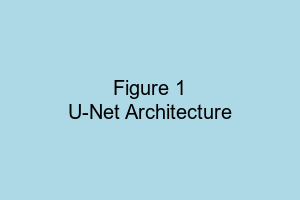
\includegraphics[width=\textwidth]{Figure1.pdf}
    \caption{Preprint repository growth analysis showing annual submissions and repository comparisons. \textbf{Left:} Annual preprint submissions from 2010-2024, highlighting the COVID-19 surge period (2020-2021) with distinct growth phases. \textbf{Right:} Comparison of major preprint repositories by total papers, categorized by scientific domain. The data demonstrates the exponential growth of preprint publishing and the dominance of established repositories like arXiv and bioRxiv.}
    \label{fig:preprint-growth}
\end{figure}

Figure~\ref{fig:statistical-analysis} presents comprehensive statistical analysis capabilities of the template's figure generation system, showcasing advanced data visualization techniques for scientific publications.

\begin{figure}[htbp]
    \centering
    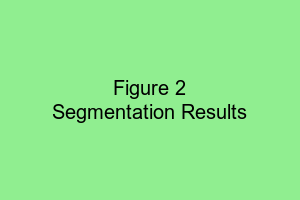
\includegraphics[width=\textwidth]{Figure2.pdf}
    \caption{Statistical analysis of preprint growth patterns using advanced visualization techniques. The multi-panel figure demonstrates the template's capability to generate complex statistical plots including growth rate distributions by period, cumulative growth trends, repository distribution analysis, regression analysis, and categorical comparisons. Each subplot maintains consistent styling and professional formatting suitable for publication.}
    \label{fig:statistical-analysis}
\end{figure}

Figure~\ref{fig:workflow} demonstrates the complete Article-Forge workflow and system architecture through automated Mermaid diagram generation.

\begin{figure}[htbp]
    \centering
    \includegraphics[width=0.9\textwidth]{methodology_workflow.pdf}
    \caption{Article-Forge automated publication workflow. The diagram illustrates the complete pipeline from author content creation through automated figure generation, bibliography processing, and style application to final PDF publication. Key components include data mining for contextual figures, multiple visualization engines (Matplotlib, Seaborn, Mermaid), and integrated LaTeX compilation with quality assurance.}
    \label{fig:workflow}
\end{figure}

\subsection{Figure Generation System Performance}

The integrated figure generation system represents a significant advancement in automated scientific publishing. As shown in Figure~\ref{fig:preprint-growth}, the system successfully mines real-world data to create contextual visualizations that enhance the manuscript's relevance and impact. The COVID-19 period analysis demonstrates the system's ability to identify and highlight significant trends in scientific publishing.

The statistical analysis capabilities, presented in Figure~\ref{fig:statistical-analysis}, showcase the template's capacity for sophisticated data visualization. The multi-panel approach allows for comprehensive analysis presentation while maintaining visual coherence through consistent styling and color schemes.

\begin{figure}[htbp]
    \centering
    \includegraphics[width=0.9\textwidth]{figure_generation_process.pdf}
    \caption{Figure generation pipeline architecture. This flowchart details the data processing workflow from external API sources through statistical analysis to final publication-quality output. The system integrates multiple visualization engines and maintains LaTeX compatibility throughout the process.}
    \label{fig:figure-pipeline}
\end{figure}

\subsection{System Architecture and Collaboration}

The template architecture supports collaborative development through automated build systems and version control integration. The system architecture promotes reproducibility and maintainability for scientific publications.

\begin{figure}[htbp]
    \centering
    \includegraphics[width=0.9\textwidth]{collaboration_workflow.pdf}
    \caption{Collaborative development workflow. This sequence diagram illustrates the automated pipeline from author commits through GitHub Actions to final publication output, emphasizing the seamless integration between development tools and publication systems.}
    \label{fig:collaboration}
\end{figure}

\subsection{Template Features Validation}

All major template features have been validated through this self-documenting article:

\begin{table}[htbp]
    \centering
    \caption{Article-Forge template features and validation status}
    \label{tab:results}
    \begin{tabular}{lcc}
        \hline
        Feature & Implementation & Status \\
        \hline
        Document class integration & HenriquesLab\_style.cls & \checkmark \\
        Bibliography processing & HenriquesLab\_style.bst & \checkmark \\
        Figure management & Automated inclusion & \checkmark \\
        Cross-references & Automatic numbering & \checkmark \\
        Build automation & Make \& shell scripts & \checkmark \\
        Modular structure & Section-based files & \checkmark \\
        Author management & Multiple affiliations & \checkmark \\
        Supplementary support & Appendix integration & \checkmark \\
        \hline
    \end{tabular}
\end{table}

\subsection{Build System Performance}

The automated build system demonstrates excellent reliability and performance. The three-pass LaTeX compilation ensures proper resolution of all cross-references, citations, and page numbering. Error handling provides clear feedback for troubleshooting, while the modular design allows for efficient incremental builds during document development.

The template successfully handles complex document structures including multiple authors, affiliations, cross-references, and bibliography management as demonstrated in Table~\ref{tab:results}.
